\section{Solutions}
%Project workflow
\begin{frame}[shrink]{Project workflow}
	\begin{figure}	
		\begin{tikzpicture}
		\tikzstyle{block} = [rectangle, draw, fill=blue!20,minimum height=1cm,text badly centered]
		\tikzstyle{line} = [draw,ultra thick, -latex']	
		\uncover<1->{\node[block,text width=22em] (entrance){
				\begin{tabular}{@{}c|c|c@{}}
				\multicolumn{3}{c}{Channel near river mouth}\\
				\midrule
				N, P&Plant&Vegetation\\
				accumulation&comprehensive&patterns\\
				ability&evaluation&construction\\ \cline{1-2}
				\multicolumn{2}{|c|}{Plant selection}&\\ \cline{1-2}
				\end{tabular}
			};}
		
		\uncover<2->{\node[block,text width=17em] at(7.9,0.24) (around){
				\begin{tabular}{@{}p{5em}|p{10em}@{}}
				\multicolumn{2}{c}{Area around reservoir}\\
				\midrule
				Wetland modification&Relationship between stand structure and conservation capacity\\
				\end{tabular}
			};
		}	
		
		\uncover<3->{
			\node[block,text width=42em] at(3.5,-3.9) (teches){
				\begin{tabular}{@{}p{13em}|p{13em}|p{13em}@{}}		
				Technology of restoring riparian vegetation	& Technology of reforming and conserving wetland & Technology of adjusting and improving conservation stand structure\\
				\end{tabular}
			};	
		}
		
		\uncover<4->{
			\node[block,text width=42em] at(3.5,-6.5) (techintegrated){
				\begin{tabular}{@{}c p{39em}@{}}		
				Technology of optimizing riparian vegetation composition and spatial structure\\
				\end{tabular}
			};
		}	
		
		\uncover<5->{	
			\node[block,text width=42em] at(3.5,-8.7) (demo){
				\begin{tabular}{@{}c p{39em}@{}}		
				Demonstration projects of restoration of riparian vegetation\\
				\end{tabular}
			};
		}
		
		% Draw arrows
		\uncover<3->{
			\path [line] (entrance) -- (4.4,0) -- (4.4,-3);
			\node[left] at (4.4,-2.3) {Water quality improvement};
			\node[right] at (4.4,-2) {Vegetation restoration};
			\path [line] (4.8,0) -- (4.4,0) -- (4.4,-3);	
		}
		
		\uncover<4->{\path [line] (teches) -- (techintegrated);
			\node[right] at (3.5,-5.4) {Technology integration};
		}
		
		\uncover<5->{
			\path [line] (techintegrated) -- (demo);
			\node[right] at (3.5,-7.6) {Application};
		}
		
		\end{tikzpicture}
		\caption{Project workflow.}
	\end{figure}
\end{frame}

%N, P accumulation ability of the plants
\begin{frame}{Experiments on N, P accumulation ability}
\begin{columns}[T,onlytextwidth]
	\column{0.4\textwidth}
	\begin{table}
		\caption{Experimental plants}
		\begin{tabular}{p{3em}|p{3em}}		
			\toprule		
			Plant&Number\\		
			\midrule
			Tree&27\\
			\textcolor{colshrub}{Shrub}&21\\
			\textcolor{colherb}{Herb}&20\\
			Total&68\\		
			\bottomrule
		\end{tabular}
	\end{table}
\vspace{0.5cm}	
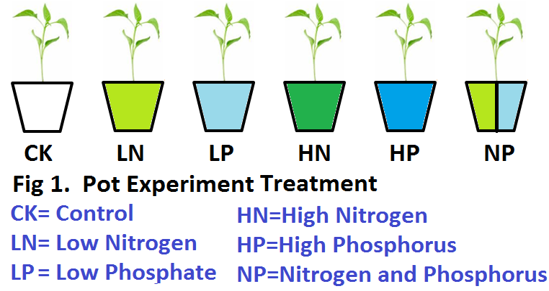
\includegraphics[width=\textwidth]{NP_experimental_design.png}
%\column{0.01\textwidth}
\column{0.6\textwidth}
\begin{table}
	\caption{Experimental design}
	\begin{tabular}{p{3em}|p{1.5em}|p{1.5em}}		
		\toprule
		%			Treat\newline ment&TN\newline (mg/L)&TP\newline (mg/L)\\
		Treat-&TN&TP\\
		ment&\multicolumn{2}{c}{(mg/L)}\\
		\midrule
		LN&14&0\\
		HN&56&0\\
		LP&0&3\\
		HP&0&12\\
		NP&14&3\\
		\bottomrule
	\end{tabular}
\end{table}	
\begin{columns}[b,onlytextwidth]
	\column{0.835\textwidth}
	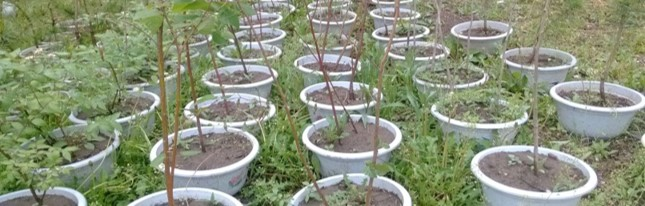
\includegraphics[width=\textwidth]{pot_experiment_tree.jpg}
	\column{0.165\textwidth}
	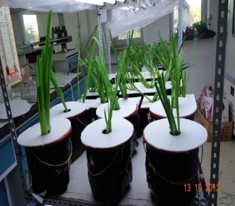
\includegraphics[height=0.2\textheight]{pot_experiment_herb.jpg}	
\end{columns}

\end{columns}
\end{frame}


%N, P accumulation ability of the plants
\begin{frame}{N, P accumulation ability of the plants}
\begin{figure}
	\centering
	\begin{columns}[T]
	\column{0.5\textwidth}
	\subfigure{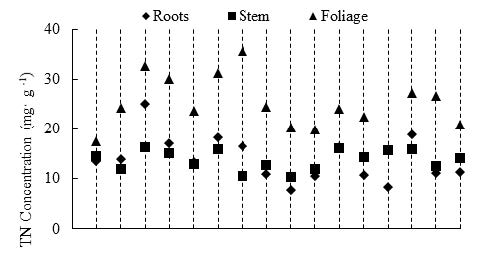
\includegraphics[width=\textwidth,height=0.3\textheight]{TN-p.jpg}}
	\subfigure{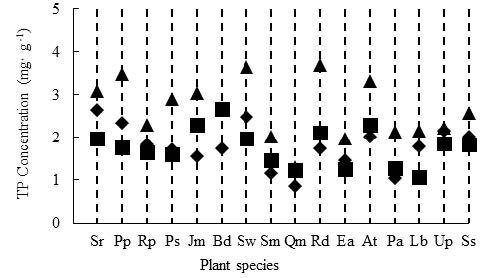
\includegraphics[width=\textwidth,height=0.3\textheight]{TP-p.jpg}}	
	%	\column{{0.01\textwidth}}
	\column{0.5\textwidth}
	\subfigure{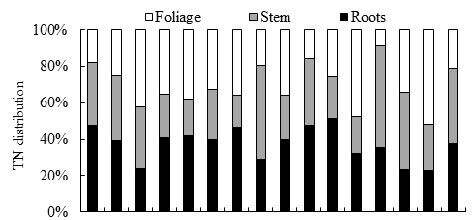
\includegraphics[width=\textwidth,height=0.3\textheight]{TN.jpg}}
	\subfigure{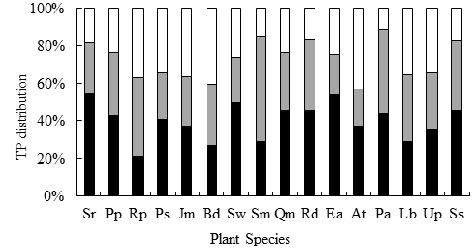
\includegraphics[width=\textwidth,height=0.3\textheight]{TP.jpg}}	
\end{columns}
\caption{Concentration and distribution of total nitrogen (TP) and total phosphorus (TP) in plants \cite{yu2014biomass}.}
%Syringa reticulate (Sr), Prunus padus (Pp), Robinia pseudoacacia (Rp), Pterocarya stenoptera (Ps), Juglans mandshuriea (Jm), Berberis dielsiana (Bd), Sambucus williamsii, Salix matsudana (Sm), Quercus mongolica (Qm), Rosa davurica (Rd), Euonymus alatus (Ea), Acer truncatum (At), Populus alba (Pa), Lespedeza bicolor (Lb), Ulmus pumila (Up) and Sorbaria sorbifolia (Ss). 

\end{figure}
\end{frame}

%Plant selection protocol (Analytic Hierarchy Process)
\begin{frame}[t]{Plant selection protocol (Analytic Hierarchy Process)}
\footnotesize
\begin{table}
	\centering
	\begin{tabular}{clrrrr}
		\toprule
		
		& \parbox[t]{2mm}{\multirow{2}{*}{\rotatebox[origin=c]{90}{Criteria}}} & A-B & \multirow{2}{*}{Index} & B-C & A-C\\
		&& $W_i$ & & $W_{ij}$ & TW\\		
		\midrule
				
		\parbox[t]{2mm}{\multirow{15}{*}{\rotatebox[origin=c]{90}{Comprehensive evaluation index (A)}}} & \parbox[t]{2mm}{\multirow{5}{*}{\rotatebox[origin=c]{90}{Resistance ($B_1$)}}} &\parbox[t]{2mm}{\multirow{5}{*}{\rotatebox[origin=c]{90}{0.47}}}&Cold tolerance (C11)&0.31&0.14\\		
		& &&Poor soil tolerance (C12)&0.12&0.05\\
		& &&Shade tolerance (C13)&0.23&0.10\\
		& &&Flooding tolerance (C14)&0.24&0.11\\		
		& &&Drought tolerance (C15)&0.11&0.05\\	\cline{2-6}	
		
		& \parbox[t]{2mm}{\multirow{5}{*}{\rotatebox[origin=c]{90}{Ecological ($B_2$)}}} &\parbox[t]{2mm}{\multirow{5}{*}{\rotatebox[origin=c]{90}{0.44}}}&N absorbing ability (C21)&0.23&0.10\\		
		& &&P absorbing ability (C22)&0.21&0.11\\
		& &&Biomass accumulation (C23)&0.38&0.18\\
		& &&Water conservation ability (C24)&0.09&0.04\\
		& &&Soil conservation ability (C25)&0.10&0.05\\	\cline{2-6}		
		
		& \parbox[t]{2mm}{\multirow{5}{*}{\rotatebox[origin=c]{90}{Aesthetic ($B_3$)}}} &\parbox[t]{2mm}{\multirow{5}{*}{\rotatebox[origin=c]{90}{0.08}}}&Leaf shape (C31)&0.20&0.02\\		
		& &&Flower shape (C32)&0.09&0.01\\
		& &&Fruit shape (C33)&0.08&0.01\\
		& &&Canopy shape (C34)&0.43&0.04\\
		& &&Shape in winter (C35)&0.20&0.02\\
				
		\bottomrule
	\end{tabular}
\end{table}
\tiny
A--B: $\lambda_{max}$ = 3.0037, CI = 0.0036, RI1 = 0.58, CR = 0.0620 $<$ 0.1; 
$B_1$--C: $\lambda_{max}$ = 5.4118, CI1 = 0.0919, RI1 = 1.12, CR1 = 0.0820 $<$ 0.1\\
$B_2$--C: $\lambda_{max}$ = 5.2180, CI2 = 0.0587, RI2 = 1.12, CR2 = 0.0524 $<$ 0.1; 
$B_3$--C: $\lambda_{max}$ = 5.3876, CI3 = 0.0865, RI3 =1.12, CR3 = 0.0772 $<$ 0.1\\
Total rank: CI = $W_1*CI1 + W_2*CI2 + W_3*CI3$ = 0.0349, RI = $W_1*RI1 + W_2*RI2 + W_3*RI3$ = 0.8651, CR = 0.0403 $<$ 0.1\\
\normalsize
\end{frame}

%List of selected plants
\begin{frame}{List of selected plants}
%\footnotesize
\scriptsize
%\tiny
\begin{columns}[T,onlytextwidth]
	\metroset{block=fill}
	\column{0.33\textwidth}
	\begin{block}{Tree}
	\begin{enumerate}
		\item \emph{Ulmus pumila} \item \emph{Syringa reticulate} \item \emph{Salix matsudana}
		\item \emph{Robinia pseudoacacia} \item \emph{Salix babylonica} \item \emph{Juglans mandshurica}
		\item \emph{Berberis dielsiana} \item \emph{Morus alba} \item \emph{Fraxinus mandschurica}
		\item \emph{Acer mono}		
	\end{enumerate}	
	\end{block}
	
	\column{0.33\textwidth}
	\begin{alertblock}{Shrub}
		\begin{enumerate}			
			\item \emph{Lespedeza bicolor} \item \emph{Lonicera chrysantha} \item \emph{Sambucus williamsii}
			\item \emph{Sorbaria sorbifolia} \item \emph{Amorpha fruticose} \item \emph{Salix viminalis}
			\item \emph{Acer ginnala} \item \emph{Salix integra} \item \emph{Flueggea suffruticosa}
			\item \emph{Euonymus maackii}		
		\end{enumerate}	
	\end{alertblock}
	
	\column{0.33\textwidth}
	\begin{exampleblock}{Herb}		
		\begin{enumerate}			
			\item \emph{Phragmites australis} \item \emph{Artemisia capillaris} \item \emph{Sparganium stoloniferum}
			\item \emph{Impatiens noli-tangere} \item \emph{Polygonum persicaria} \item \emph{Iris pseudacorus}
			\item \emph{Acorus tatarinowii} \item \emph{Monochoria korsakowii} \item \emph{Iris sanguinea}
			\item \emph{Lythrum salicaria}
		\end{enumerate}	
	\end{exampleblock}	
\end{columns}
\end{frame}


%Effects of stand structure on biodiversity and water-holding capacity
\begin{frame}{Effects of tending intensity on species diversity and water-holding capacity of WCS}
\begin{table}
	\caption{Effects of tending intensity on species diversity and water-holding capacity of water-conservation stands (WCS)}
	\begin{tabular}{@{}l@{}|@{}cccccc@{}|@{}cc@{}}
		\toprule
		\multirow[c]{3}{4ex}{Treat-ment} & \multicolumn{6}{c}{Species number} & \multicolumn{2}{|c}{Water}\\
		&\multicolumn{3}{c}{First year} & \multicolumn{3}{c}{Second year}& \multicolumn{2}{|c}{storage ($t/hm^2$)}\\
		&  Tree &\textcolor{colshrub}{Shrub} &\textcolor{colherb}{Herb}&Tree&\textcolor{colshrub}{Shrub}&\textcolor{colherb}{Herb}&Total& Non-capillary\\
		\midrule
		CK&14&7&3&15&7&3&1022&220\\
		Weak&15&7&3&16&8&3&1054&260\\
		Medium&16&8&4&18&8&4&1085&295\\
		Intense&18&8&4&20&10&5&1100&324\\
		\bottomrule
	\end{tabular}
\end{table}
\end{frame}

%Technology of restoring riparian vegetation near river mouth
\begin{frame}{Technology: restore riparian vegetation near river mouth}
\vspace{-0.2cm}
\begin{columns}[T,onlytextwidth]
	
	\column{0.40\textwidth}	
	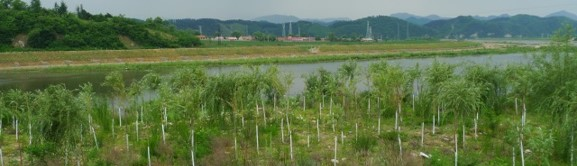
\includegraphics[height=1.5cm]{veg_pattern_construction.jpg}
	
	\column{0.20\textwidth}
	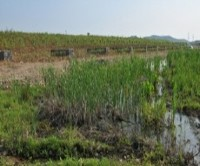
\includegraphics[height=1.5cm]{macrophyte.jpg}
	
	\column{0.20\textwidth}
	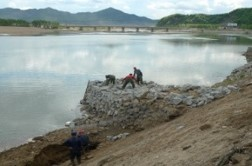
\includegraphics[height=1.5cm]{gabion_spur_dike.jpg}
	
	\column{0.20\textwidth}
	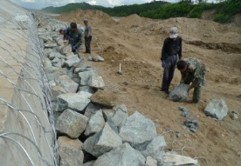
\includegraphics[height=1.5cm]{gabion_revetment.jpg}
\end{columns}
\vspace{-0.2cm}
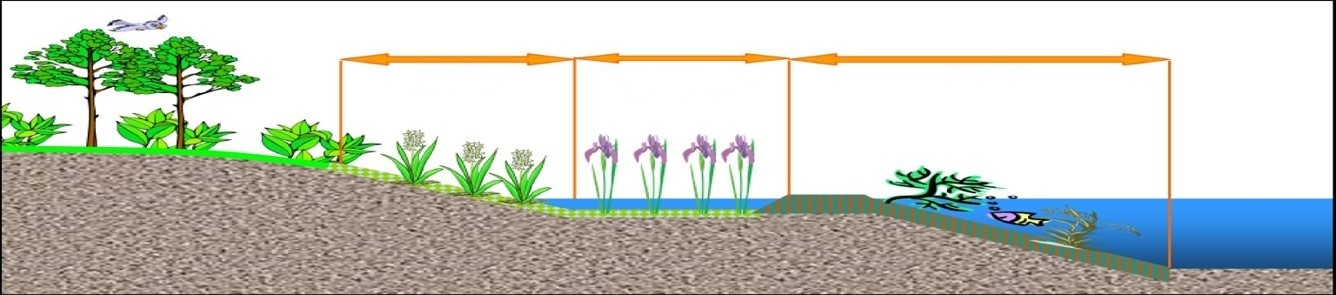
\includegraphics[width=\textwidth]{veg_resto_near_entrance.jpg}

%\end{frame}
%
%\begin{frame}{cont}
\vspace{-0.4cm}
\begin{columns}[T,onlytextwidth]
	
	\column{0.7\textwidth}
	%\hspace{0.2cm}
	\begin{itemize}
		\small
		\item Reservoir shoal:\\
		\tiny
		\emph{Salix viminalis}, \textcolor{colherb}{\emph{Iris sanguinea}}, \textcolor{colherb}{\emph{Phragmites australis}}, \textcolor{colherb}{\emph{Sparganium stoloniferum}}, \textcolor{colherb}{\emph{Artemisia capillaris}}, \textcolor{colherb}{\emph{Polygonum persicaria}}\\
		%\emph{}
		%	\textcolor{colherb}{\emph{}},
		%\textcolor{colshrub}{\emph{}},
		\small
		\item Barren area:\\
		\tiny
		\emph{Salix viminalis}, \textcolor{colshrub}{\emph{Lespedeza bicolor}}, \textcolor{colshrub}{\emph{Sorbaria sorbifolia}}, \textcolor{colherb}{\emph{Artemisia capillaris}}, \textcolor{colherb}{\emph{Polygonum persicaria}}, \textcolor{colherb}{\emph{Iris sanguinea}}\\
		
		\small
		\item Flat fertile area:\\
		\tiny
		\emph{Juglans mandshurica}, \emph{Fraxinus mandschurica}, \emph{Ulmus pumila}, \textcolor{colshrub}{\emph{Sorbaria sorbifolia}}, \textcolor{colshrub}{\emph{Lonicera chrysantha}}, \textcolor{colshrub}{\emph{Sambucus williamsii}}, \textcolor{colherb}{\emph{Impatiens noli-tangere}}, \textcolor{colherb}{\emph{Sparganium stoloniferum}}, \textcolor{colherb}{\emph{Iris pseudacorus}}, \textcolor{colherb}{\emph{Phragmites australis}}, \textcolor{colherb}{\emph{Monochoria korsakowii}}, \textcolor{colherb}{\emph{Lythrum salicaria}}\\
		
		\small
		\item Steep hilly area:\\
		\tiny
		\emph{Salix viminalis}, \emph{Berberis dielsiana}, \emph{Robinia pseudoacacia}, \emph{Salix babylonica}, \emph{Syringa reticulate}, \textcolor{colshrub}{\emph{Amorpha fruticosa}}, \textcolor{colshrub}{\emph{Sorbaria sorbifolia}}\\
	\end{itemize}
	
	\column{0.3\textwidth}
        \small
	\begin{table}
		%\caption{Plant parameters}
		\begin{tabular}{p{5em}| p{5em}}
			\toprule
			Vegetation type&Distance/ density\\
			\midrule
			Tall tree&4--6 m\\
			Dwarf tree&2--3 m\\
			\textcolor{colshrub}{Shrub}&1--2 m\\
			\textcolor{colherb}{Herb}&0.4--1.2 m\\
			\textcolor{colherb}{Macrophyte}&2--10  / $m^2$\\
			\bottomrule
		\end{tabular}
	\end{table}
		
\end{columns}
\end{frame}

%Technology of reforming and conserving wetland around the reservoir
\begin{frame}{Technology: reform and conserve wetland around reservoir}
\vspace{-0.1cm}
\begin{columns}[T,onlytextwidth]
	
	\column{0.20\textwidth}	
	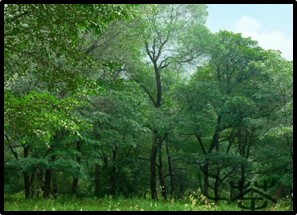
\includegraphics[height=1.5cm]{wetland_tree_r2.jpg}
	
	\column{0.15\textwidth}
	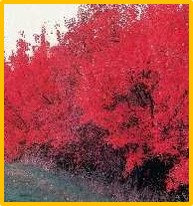
\includegraphics[height=1.5cm]{wetland_shrub_r1.jpg}
	
	\column{0.20\textwidth}
	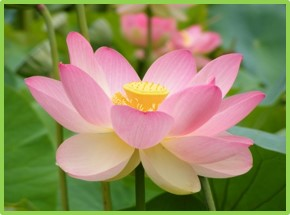
\includegraphics[height=1.5cm]{wetland_buff_zone_herb_r4.jpg}
	
	\column{0.1\textwidth}
	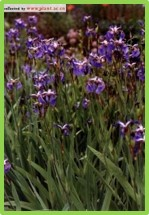
\includegraphics[height=1.5cm]{wetland_buff_zone_herb_r1.jpg}

        \column{0.12\textwidth}
	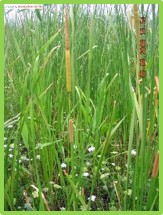
\includegraphics[height=1.5cm]{wetland_herb_r5.jpg}

        \column{0.11\textwidth}
	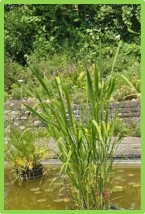
\includegraphics[height=1.5cm]{wetland_herb_r3.jpg}

        \column{0.11\textwidth}
	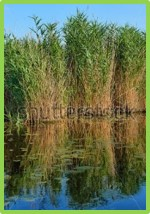
\includegraphics[height=1.5cm]{wetland_herb_r2.jpg}
\end{columns}
\vspace{-0.3cm}
\footnotesize
\begin{table}
  \begin{tabular}{p{12em}|p{8em}|p{9em}|p{4em}}
    \toprule
    Ecological protection zone&Buffer zone&Shoal&Reservoir\\
    Terrestrial&Water 40--90 cm& Water $<$ 40 cm&\\
    Partial fenced area&Buffer ponds&Littoral zone&\\
    \midrule
    \emph{Ulmus pumila}&\textcolor{colherb}{\emph{Nelumbo nucifera}}&\textcolor{colherb}{\emph{Scirpus validus}}&\\

    \emph{Fraxinus mandschurica}&\textcolor{colherb}{\emph{Alisma plantago}}&\textcolor{colherb}{\emph{Typha angustifolia}}&\\

    \textcolor{colshrub}{\emph{Acer ginnala}}&\textcolor{colherb}{\emph{Lythrum salicaria}}&&\\

&\textcolor{colherb}{\emph{Iris sanguinea}}&&\\    
    \bottomrule
  \end{tabular}
\end{table}
\vspace{-0.3cm}
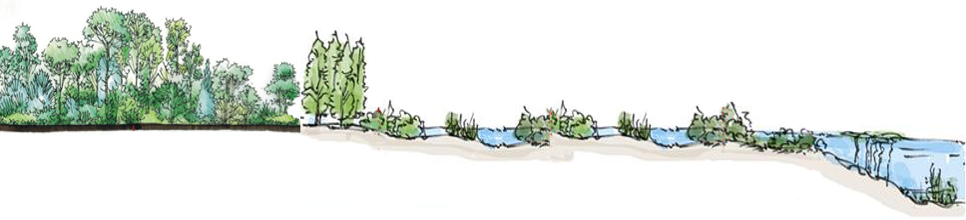
\includegraphics[width=\textwidth]{wetland_veg_structure.png}

\end{frame}

%Technology of adjusting and improving structure of water-conservation-stands
\begin{frame}{Technology: adjust and improve structure of WCS}
  \vspace{-0.2cm}
  \begin{columns}[T,onlytextwidth]
    \scriptsize
    \column{0.65\textwidth}
    \metroset{block=fill}
    \begin{exampleblock}{Chinese pine (\emph{Pinus tabulaeformis}) stand:}
      \begin{itemize}
      \item Block thinning
      \item Interplant distance 3.5 m
      \item Forest gap 10--15\%
      \item Dominant with young and mid-aged trees
      \end{itemize}      
    \end{exampleblock}
    \vspace{-0.3cm}
    \begin{exampleblock}{Larch (\emph{Larix gmelinii}) stand:}
      \begin{itemize}
      \item Selection-felling with strip reform
      \item Replant Chinese pine and local broadleaf trees
      \item Canopy density 0.5--0.7
      \item Mixed coniferous forest dominant with trees and shrubs
      \end{itemize}      
    \end{exampleblock}
    \normalsize
    \column{0.01\textwidth}
    \column{0.34\textwidth}
    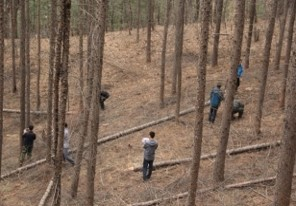
\includegraphics[width=\textwidth,height=2.7cm]{selection_felling.jpg}
      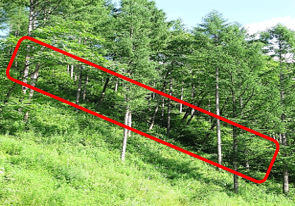
\includegraphics[width=\textwidth,height=2.7cm]{strip_reform.png}
  \end{columns}
  % \vspace{-0.1cm}
  \vspace{0.2cm}
  \begin{columns}[T,onlytextwidth]
    \column{0.33\textwidth}
%    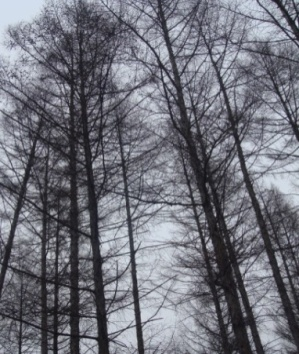
\includegraphics[width=\textwidth]{wcs_before_2010.png}
      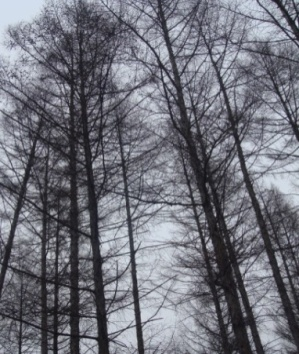
\includegraphics[width=\textwidth,height=2.5cm]{wcs_before_2010.png}
  \column{0.33\textwidth}
%  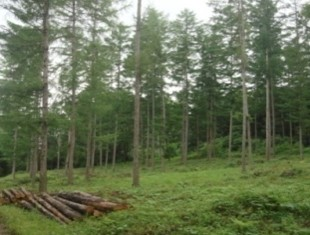
\includegraphics[width=\textwidth]{wcs_thinning_2012.jpg}
  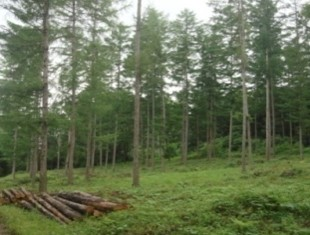
\includegraphics[width=\textwidth,height=2.5cm]{wcs_thinning_2012.jpg}
    \column{0.33\textwidth}
%    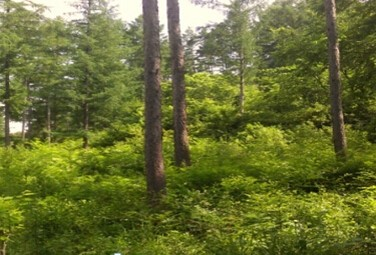
\includegraphics[width=\textwidth]{wcs_after_2015.jpg}
    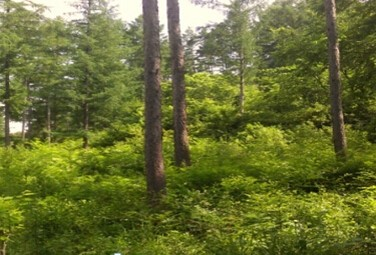
\includegraphics[width=\textwidth,height=2.5cm]{wcs_after_2015.jpg}
  \end{columns}  
\end{frame}